\documentclass[10pt, a4paper]{article}
\usepackage{graphicx}
\usepackage{geometry}
 \geometry{
 a4paper,
 total={170mm,257mm},
 left=20mm,
 top=20mm,
 }
 
\title{Are temperatures of one year significantly correlated with the next year}

\author{Junyue Zhang}

\date{01-16-2022}

\begin{document}
  \maketitle
  
  \section{Results}
    The correlation coefficient between successive years is calculated as 0.326. And this calculation is repeated 10000 times, each time the time series of annual temperatures is randomly permuted, and the correlation coefficient is recalculated. The random correlation coefficients are continuously appended in a new vector. Then the fraction of the random correlation coefficient greater than 0.326 is considered as the approximate, asymptotic p-value. 
    Thus, the p-value is calculated as zero.  
   
  \section{Discussion}
    The p-value indicates the probability that the occurrence of an observed difference just by random chance. The lower p-value is related to the greater statistical significance of the observed difference.
    In this case, the p-value is less than 0.01, which means the difference between successive years is significant.
    It can be speculated that the temperature of one year is significantly correlated with the next year across years in Florida.  
    Therefore, temperatures of one year are significantly correlated with the successive years in Florida.

  \section{Conclusion}
    After applying a distribution of random correlation coefficients in temperatures between successive years, it can be concluded that temperatures of one year are significantly correlated with the successive years in Florida.

\begin{figure}[h]
  \centering
  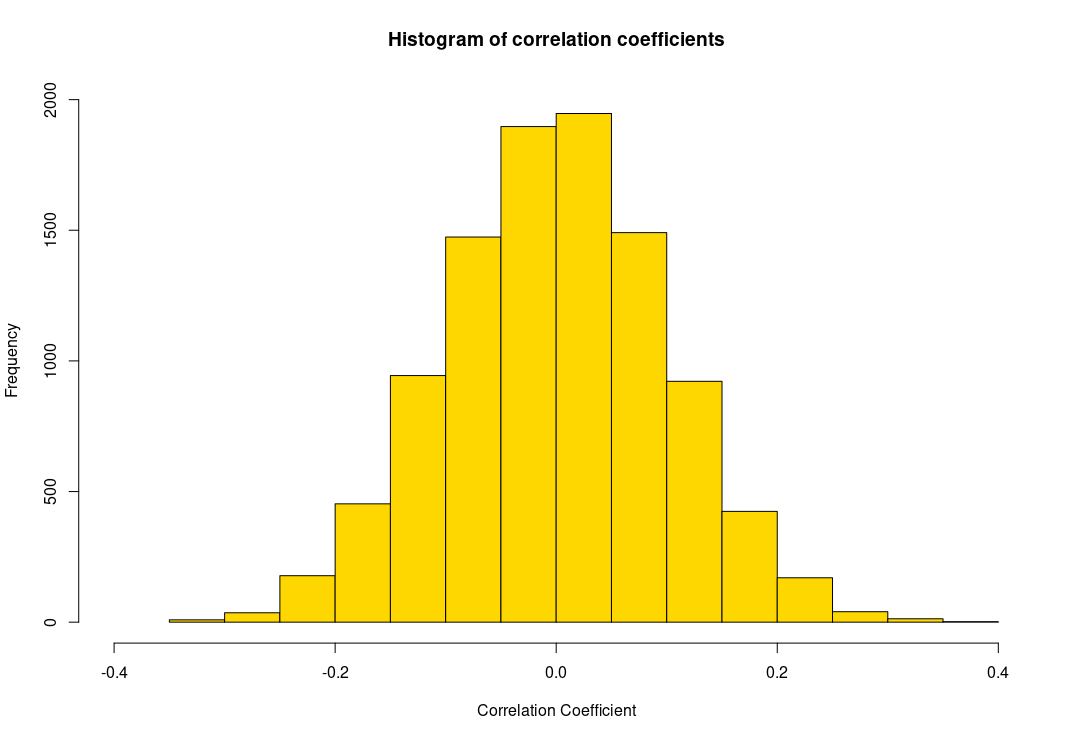
\includegraphics[scale = 0.3]{./Hist.png}
  \caption{Histogram of Correlation Coefficients}
  \label{figure1}
\end{figure}
Figure \ref{figure1} shows a histogram of correlation coefficients.

\end{document}